% Auditable Model Routing — Layer 5 full paper draft (HBR register)
% Thesis updated 2026-10-25 after the owner's decision that privacy and the model list
% belong to the user. Numbers are produced by experiments/spine.py (exit 0, 263 checks — see
% experiments/results/derived/verification_summary.json).
\documentclass[11pt]{article}
\usepackage[margin=1in]{geometry}
\usepackage{booktabs}
\usepackage{graphicx}
\usepackage{hyperref}
\usepackage{microtype}
\usepackage{xcolor}
\usepackage{amssymb}
\usepackage{array}
\graphicspath{{figures/}}
\newcommand{\ev}{\ensuremath{\blacktriangleright}}
\newcommand{\code}[1]{\texttt{#1}}
\title{Auditable Model Routing: Policy as Data,\\Decisions as Evidence\\[4pt]
\large the routing layer of DeeWaanAI OS}
\author{Youssef Hariri\\DeeWaanAI\\\texttt{github.com/DeeWaanAI}}
\date{October 2026}

\begin{document}
\maketitle

\begin{abstract}
Every assistant now routes: a request is classified, a model is chosen, and the choice is
explained by code nobody can re-run. We argue that the routing layer itself should be the
auditable object, and we build one. The policy --- gate order, thresholds, prices, allowed
data loci --- lives in bound datasets, not code; every decision is written as one record
carrying its classifier output, the full gate trace, the feasible set with its cost for each
candidate, and a claim binding whose sources resolve. A replay audit rebuilds the registry as
it stood at each decision's timestamp and recomputes the trace, the winner and its cost;
\textbf{263 checks pass on 414 recorded decisions across eight runs}, including every
decision that spent money. Because
eligibility is a \emph{measurement}, we freeze a capability matrix from frozen runs and show
that moving two thresholds changes which model answers and what it costs, with no code change:
on six computation items the same frozen measurements route to a free 3B model (measured
accuracy 0.00), a free 8B (0.67), a \$1.04/Mtok model (0.83) or a \$2/\$6 model (1.00)
depending only on the policy. On the task that motivated the design, \textbf{four of five models
compute an 800-row total exactly when they write and run code, and none of those that can fit the
rows in context compute it there}. We are equally explicit about what the layer cannot promise: privacy is a
user-declared policy, not a property of the architecture; with 6 items per capability cell one
correct answer flips a verdict; and our own answer-key defect was found by the audit, not by the
experiment. We test the audit itself by injecting seven corruptions, six of them written through the
store with a valid hash chain; \textbf{all seven are caught on the check that should catch
them, with no false alarms on clean copies}. Against five fixed strategies the router is not
dominated: a free local model reaches 0.73 accuracy at \$0, the most expensive arm reaches 1.00
for 4.8$\times$ what the router pays for the same score, and one tie-break defect --- found by
the baseline, not by inspection --- silently selected an unmeasured model at identical cost.
The contribution is not a better router --- it is a router whose every claim, including the
uncomfortable ones, can be recomputed, and whose audit has been shown to fail when it should.
\end{abstract}

\section{Introduction}

A modern assistant does not answer with one model. It decides: is this request private, what
kind of task is it, which models are good enough, what does each cost, which endpoint is alive
--- and then it answers, or refuses, or falls back. That decision is now the interesting part of
the system, and it is almost always invisible. Policies live in configuration files, feature
flags and if-statements; the record of why a request went to a model is a log line saying which
model ran. When the answer is wrong, or the bill is high, or a regulator asks, nobody can
reconstruct the decision, because the inputs are gone and the code has moved.

This paper takes the opposite position: \textbf{the routing decision should be the auditable
artifact}. A request's route is a claim about the world --- \emph{this was the cheapest suitable
model, under this policy, with this evidence} --- and a claim should carry its proof. We build
that layer and we test the claim the way a skeptic would: by recomputing every number from
frozen artifacts, with a separate script, and failing when the two disagree.

\paragraph{Contributions, stated as claims.}
\begin{enumerate}
\item \textbf{Policy as data.} Gates, thresholds, prices and allowed data loci are records in a
provenance substrate, not literals in code. A policy edit reroutes with no code change; the
paper measures the resulting movement in choice and cost (Section~\ref{sec:sweep}).
\item \textbf{Decisions as evidence.} Each decision stores the classifier verdict, the ordered
gate trace with the excluded set and reason for every candidate, per-candidate token estimates
and declared cost, the attempt chain with provider-metered usage, and a binding to the policy
and rulesets in force. An audit rebuilds the registry at the decision's timestamp and requires
the replay to equal the record exactly (Section~\ref{sec:replay}).
\item \textbf{Verifiability as a measured constraint.} Capability rows come only from frozen
runs; eligibility is computed twice, from the row's own snapshot and from the current policy, so
an old measurement cannot silently change meaning. Unmeasured pairs are counted, not hidden
(Section~\ref{sec:eligibility}).
\item \textbf{Failure is part of the contract.} Typed connector errors, bounded retries on
transient classes only, a per-connection circuit breaker, fallback inside the feasible set, one
record even when everything fails, and an append lock that keeps the chained history intact
under concurrency. All of it is tested against a real HTTP server with switchable failures
(Section~\ref{sec:resilience}).
\end{enumerate}

\paragraph{What this paper does not claim.} It does not claim that the router protects privacy.
It does not claim state-of-the-art routing quality. It does not claim statistical power it does
not have. Section~\ref{sec:limits} is unusually long on purpose.

\section{Background: the Qafiya substrate}

Qafiya is a provenance-first data substrate: every dataset lives as an append-only JSONL file
with a schema, a hash-chained history, bindings, and a quarantine list for artifacts that were
\emph{wrong} (as opposed to merely old, which are superseded by succession). A binding is a
first-class claim about a record: what was measured, by which derivation, with which sources,
and what the claim asserts on both sides of a comparison. Ids are prefixed and sortable; nothing
is deleted; a record is retired by writing its successor and pointing at it.

Layer 5 uses five datasets: \code{models} (the user's connect list), \code{capabilities}
(measured per model and task class), \code{policy} (gates, thresholds, objective),
\code{rules} (classifier rulesets) and \code{decision\_log}. The substrate supplies the chain
and the §8 layout; this layer supplies the decision semantics. The distinction matters because
the paper's central property --- replay against the registry \emph{as it stood} --- is only
possible if the registry has a history, and only useful if a decision cannot be quietly rewritten
after the fact.


\section{Related work}\label{sec:related}

\paragraph{Cascades and routing.} The field opened with sequential cascades: try a cheap model,
escalate when a scorer doubts the answer, and report large cost reductions at matched quality
\cite{frugal,mot}. Two-model routers followed, trained on preference data \cite{routellm} or as a
quality-aware binary decision \cite{hybrid}, with self-verification driving the mix
\cite{automix} and agreement between cheap models acting as the escalation signal
\cite{agreement}. A unifying analysis shows that routing and cascading are points on one design
space rather than different mechanisms \cite{unified}. Benchmarks made the comparison
reproducible \cite{routerbench}, and a recent anatomical study finds that coarse task identity
explains most of what routers learn \cite{tasktype} --- a result this paper leans on, since our
eligibility gate is exactly a per-task-class measurement.

\paragraph{Privacy in routing.} Privacy appears in this literature as a penalty term inside the
cost objective, or as a cascade policy trained with privacy in the loop
\cite{privcascade}, or as an architectural split between edge small models and cloud large ones
\cite{edgesurvey}. None of these treats the data locus as a hard, pre-network set filter whose
verdict is recorded per decision. Our layer does, while leaving the policy itself to the user
(§\ref{sec:design}).

\paragraph{Auditability and verification.} The closest work to our thesis is a proposal for
deterministic, auditable routing in regulated environments \cite{auditroute}, and VeriRouter,
which makes routing decisions checkable \cite{verifier}. We differ in mechanism and in scope: the
decision is a bound record in a provenance substrate, replayable against the registry as it stood,
and the audit itself is evaluated by fault injection (§5). The failure literature motivates that
choice: routers can be steered toward expensive models by adversarial suffixes \cite{rome}, and
models that are selectable can still be unusable for a structured-output class
\cite{structout} --- the second is the hazard our verifiability gate measures rather than assumes.


\section{Design}\label{sec:design}

\subsection{A decision is one record, written once}

Routing produces exactly one record per request. It contains the classifier's verdict and the
rule rank that produced it (so a classifier change is visible in the record and not only in the
code), the ordered gate trace, the feasible set, the attempt chain, the outcome, and a binding
id. Records are never updated: a correction is a new record plus a succession, and the history
chain records both. The prompt itself is not stored; the record holds a keyed HMAC, so a leak
scan can look for exact text without the log becoming a corpus of user content.

The record is also the response. The caller receives the outcome, the chosen connection, the
attempt chain with error classes, and \emph{two} cost numbers kept deliberately apart: the
list-price estimate computed from declared prices, and the actual spend reported by provider
meters. Conflating those two is the most common way a routing paper overstates its savings;
we refuse to do it.

\subsection{Four gates, and a refusal that names its reason}

Gates run in the order the policy declares:

\begin{enumerate}
\item \textbf{Privacy.} Compares the request's class against the declared locus and the declared
visibility of each connection. A class with no mapping fails closed.
\item \textbf{Availability.} Removes endpoints the circuit breaker has opened
(Section~\ref{sec:resilience}).
\item \textbf{Verifiability.} Removes connections whose measured capability, under the
\emph{current} thresholds, does not clear the bar for this task class
(Section~\ref{sec:eligibility}).
\item \textbf{Context fit.} Per-connection token estimate plus expected output must fit the
declared window with a margin; an optional RAM sub-check applies only where the user declared a
budget.
\end{enumerate}

If a gate empties the set, the outcome is a typed refusal naming the gate and, in the trace, the
reason for each excluded candidate. Refusal is a first-class outcome, not an exception, and it
is recorded with the same rigour as an answer. In the experiments below there were zero refusals
on the battery, because the local window was never the binding constraint --- a fact we report
rather than omit.

\subsection{Eligibility is a measurement, not a judgement}
\label{sec:eligibility}

A capability row is (connection, task class, sample size) together with accuracy, termination
rate and schema compliance measured on a frozen battery, plus the thresholds in force when it
was written. Two verdicts are computed from it, deliberately:

\begin{itemize}
\item \emph{stored} eligibility, recomputed from the row's own \code{thresholds\_snapshot}, so an
auditor can prove the row was internally consistent when written;
\item \emph{routing} eligibility, recomputed from the policy's current thresholds, so a policy
change takes effect immediately without touching a measurement.
\end{itemize}

Neither path evaluates an expression taken from data: a row names a derivation from a closed
registry, and the audit rejects unknown names. Coverage --- measured pairs over feasible pairs
--- is a first-class number. The reason is empirical: with a sparse matrix, a strict threshold
does not produce caution, it produces \emph{fall-through} to exactly the arms nobody measured.

\subsection{Cost is declared, and nothing else}

A connection's price is declared by the user and may be zero, which is what a local model
actually costs in API terms. We deliberately do \emph{not} add a shadow price for local
electricity or for the user's waiting time: that is a valuation the router has no standing to
invent, and it silently changes which model wins. Among feasible connections the rule is the
lowest declared cost, ties broken by id, and an unpriced connection ranks \emph{last} and is
flagged --- never given an invented number. The cost--quality frontier remains an experiment
(where local is priced at zero and any crossover is a sensitivity curve), not a hidden term in
the product's decision.

\subsection{Failure is part of the contract}
\label{sec:resilience}

A desktop app that has been closed must not cost every request a timeout. The layer therefore
implements: two declared timeouts (connect and total); at most two retries, exponential with
jitter, and only for transient classes (timeout, rate limit, server, connection) --- never for
authentication, bad request or missing model, which repetition cannot fix; a per-connection
circuit breaker (three consecutive transient failures, sixty-second cooldown, half-open on
expiry, re-admitted only by a successful real call); fallback to the next feasible connection;
and one decision record containing the whole chain. Every try's usage is recorded, so a retried
call cannot double-count cost. Appends take an exclusive file lock, because a chained history has
exactly one tail and two concurrent writers would fork it.

\subsection{Two connectors, and a boundary}

Two wire formats cover the field: the OpenAI chat-completions protocol, which local runtimes
(LM Studio, Jan, GPT4All, llama.cpp server, vLLM, Ollama's \code{/v1}) and API providers all
speak, and Ollama's native path, kept because its accounting and context options differ.
Provider quirks are data on the connection (\code{request\_params}), not branches in the routing
path. Replacing per-provider backends with this pair removed eleven files --- 1{,}132 lines, of
which 257 were the backends themselves --- from the router package.

The boundary is stated in the product, not only in the paper: a subscription to a closed desktop
app is not an API entitlement. A chat subscription exposes no endpoint, and this layer will not
drive a GUI, script a paste, or pretend to. The mapping is named so the disappointment arrives
early: the desktop app maps to its separately billed API, which the generic connector already
covers.

\subsection{Privacy: mechanism versus policy}

The layer separates two things that are usually conflated.

\emph{The mechanism} is a hard set filter that runs before any network call, applies to retries
and fallbacks, and fails closed on an unmapped class. It is verified under failure: in the
mechanism experiment a private request whose only permitted endpoint is dead is \emph{refused},
and a proof-of-absence scan over the whole log --- including the failed-attempt path --- finds no
trace of the content at the forbidden endpoint.

\emph{The policy} is the user's. Whether private content may reach a cloud endpoint at all, and
what each endpoint is declared able to see, are declarations in the record --- not judgements
this layer makes. Under the shipped default a private request may go to a cloud model; when it
does, the decision carries a warning and the audit requires that warning to be present. Where
the two declarations disagree, the stricter one wins. This is a deliberate design choice with a
cost to the paper, and we state it plainly in Section~\ref{sec:limits}: the router can prove it
followed the policy, not that the policy was wise.

\paragraph{The shipped default does not classify at all.} Because the user owns the data and the
choice of provider, the default configuration sets \code{classifier.mode = trust\_user}: the text
is not analysed for sensitivity, every request is routable, and the record carries
\code{classifier\_mode = trust\_user} so no auditor mistakes ``public'' in the log for a computed
verdict. The \code{rules} mode --- classifier, privacy gate, warning on sensitive cloud routes ---
remains available and is what the privacy experiments below measure. The reason the default is the
simpler mode is not only principle: Section~\ref{sec:annotator} shows that our rule-based
classifier is the least reliable component in the layer, and a product should not ship its weakest
part as a default gate.

\section{Implementation}

The layer is Python: a store with schema validation, chained history and atomic, file-locked
appends; four gate functions as pure functions of frozen data; a transport that maps every
failure to one of eight typed classes; two connectors; an audit; and a spine script that
recomputes every headline number from raw artifacts and exits non-zero on disagreement.

Three implementation details carry more weight than their size. First, \code{code\_fingerprint}
hashes the router source into every decision, so a decision pins the \emph{code} that produced
it and not only the data --- after keyword matching changed from substrings to word boundaries,
old decisions still resolved while the change was visible. Second, gate-3 token estimates are
per-connection and the estimation method is recorded, because a character-based bound is honest
only if it is labelled as one. Third, the audit rebuilds the registry from the history rather
than reading today's active rows, which is what makes succession compatible with auditability:
retiring a model does not invalidate the decisions that used it.

\section{Evaluation}

All numbers below are recomputed by \code{experiments/spine.py} from frozen raw artifacts; the
script exits 0 only when independent paths agree. Spend on the frozen runs is \textbf{\$0.3173};
the connector checks, the replication, two budget probes and three annotation runs bring the project
total to \textbf{\$1.352} of a \$10 cap, all of it provider-metered.

\subsection{Replay: every decision re-derives}
\label{sec:replay}

We replay 414 decisions across eight runs. For each, the audit rebuilds the registry as of the
decision's timestamp, recomputes the classifier's route through the gates, and requires the
survivor set, the exclusions, the argmin and the cost arithmetic to match the record. Table~1
summarises the audit's checks.

\begin{table}[h]
\centering
\small
\begin{tabular}{@{}p{0.62\textwidth}p{0.30\textwidth}@{}}
\toprule
\textbf{Property} & \textbf{Result} \\
\midrule
Gate trace replays exactly (all runs) & 414/414 \\
Argmin of the replay equals the recorded choice & 414/414 \\
Actual cost recomputes from tokens $\times$ pinned price & 414/414 \\
Bindings resolve to live sources; none from quarantine & 414/414 \\
Registry, capability and policy chains verify & 5/5 datasets \\
Spine recomputation of headline numbers & 263 checks, exit 0 \\
\bottomrule
\end{tabular}
\caption{Audit results. The replay is not a smoke test: it reconstructs the candidate set from
history and fails on any difference in a survivor list or an exclusion reason.}
\end{table}

\subsection{Fault injection: does the audit fail when it should?}
\label{sec:faultinj}

An audit that only ever passes proves nothing. We inject seven corruptions into throwaway
copies of the store and require the audit to fail \emph{on the check responsible}. Six are
written through the store, so their hash chain is valid --- the kind of error a buggy writer
makes, which no hash can catch. The seventh edits the data file directly and leaves the chain
untouched.

\begin{table}[h]
\centering
\small
\begin{tabular}{@{}p{0.50\textwidth}p{0.26\textwidth}p{0.16\textwidth}@{}}
\toprule
\textbf{Injected fault} & \textbf{Expected check} & \textbf{Caught} \\
\midrule
chosen model is not the argmin          & §6.1.2 replay & yes \\
gate-trace survivor list edited         & §6.1.1 replay & yes \\
attempt's actual cost inflated          & §6.1.8 cost arithmetic & yes \\
\code{eligible} contradicts its snapshot & §6.1.3 recompute & yes \\
private$\rightarrow$cloud with no warning & §6.1.7 policy & yes \\
binding source does not resolve         & §6.1.6 resolution & yes \\
data file edited, chain untouched       & §6.1.5 reconciliation & yes \\
\bottomrule
\end{tabular}
\caption{Seven of seven caught on the expected check; three unmodified copies produce zero
failures, so the detector is not simply noisy.}
\end{table}

The experiment earned its place immediately: \textbf{mutation 7 passed the audit as originally
written}. The audit verified the hash chain and then read \code{data.jsonl}, without ever
checking that the file is the one the chain describes. A record could be altered, inserted or
deleted in the file the router reads and every hash would still verify. The audit now rebuilds
each dataset from its history --- replaying \code{append} and \code{status} operations --- and
requires record-for-record equality with the file on disk. That is one line of prose and a twenty-line
function, and it was invisible until something tried to cheat. Along with the earlier findings
(a decision that pinned the data but not the code, and a cascade check that compared the wrong
attempt), this is the strongest evidence we can offer for the thesis: the audit is doing work,
not decorating the paper.

\subsection{Privacy: a mechanism result and a classifier result}

The privacy battery is 44 short prompts (18 private, 11 confidential, 15 public, 9 adversarial
camouflage), frozen before the run, with labels by a single annotator. These six runs were produced
under the \code{rules} profile --- classifier plus privacy gate --- and are \textbf{not} a description of
the shipped default, which does not classify (Section~\ref{sec:design}). They measure the mechanism
for anyone who turns the stricter profile on.

\begin{table}[h]
\centering
\small
\begin{tabular}{@{}lcccccc@{}}
\toprule
Run & M1 gate & M2 end-to-end & M3 acc. & M4 over & M5 under & M6 coverage \\
\midrule
v1 policy, substring rules    & 0 & 0/18 & 0.8182 & 7 & 1 & 0.9545 \\
v2 (no text stored)           & 0 & 0/18 & 0.8182 & 7 & 1 & 0.9545 \\
v2b (word boundaries)         & 0 & 0/18 & 0.8182 & 7 & 1 & 0.9318 \\
experimental cloud arm        & 0 & 0/18 & 0.8182 & 7 & 1 & 0.9318 \\
ruleset v2                    & 0 & 0/18 & 0.8864 & 5 & 0 & 0.9545 \\
ruleset v3 (current)          & 0 & 0/18 & 0.9318 & 3 & 0 & 1.0000 \\
\bottomrule
\end{tabular}
\caption{Privacy mechanism across six runs. M1 is a proof about the filter; M2 is the
ground-truth check. Every remaining error under the current ruleset is
over-classification --- the safe direction --- and the spine asserts that set equality.}
\end{table}

Two honest readings. First, the improvement from 0.8182 to 0.9318 was produced by editing data
(two rulesets and a matcher fix), never by relaxing a rule, and the matcher fix leaves accuracy
unchanged while changing exactly one classification. On \emph{these 44 items} every remaining
error is over-classification --- a claim that Section~\ref{sec:annotator} fails to reproduce on a
held-out battery, and reports. Second, \textbf{with 44 items this
improvement is not statistically significant}: five prompts fixed and none broken gives an exact
paired test of $p = 0.0625$. The direction is consistent and the failures are in the safe
direction, but the paper does not claim a population effect from 44 prompts, and
Section~\ref{sec:limits} says what would be needed.

The mechanism result is stronger than the classifier result and is the one we rely on: in the
strict profile, no private request reached a cloud endpoint in any run, including a run where the
only permitted endpoint was dead and the request was refused. A proof-of-absence scan over data,
history and bindings finds no occurrence of the private content anywhere in the log.

\subsection{Raters agree with the labels; the classifier does not generalise}
\label{sec:annotator}

The privacy classifier is the weakest part of the layer, and this section measures it rather than
asserting it. We built three batteries in sequence, and the sequence matters:

\begin{itemize}
\item \textbf{tuning} (124 items): the original 44 plus 80 written while the rules were being revised;
\item \textbf{battery A} (64 items), written after the ruleset was frozen;
\item \textbf{battery B} (72 items), written after the guard that battery A motivated, in domains the
rules had never seen (construction, non-profits, utilities, retail, recruitment, medical billing,
legal aid, school administration, insurance, logistics).
\end{itemize}

Two independent annotators from different model families labelled everything without seeing the
rules.

\begin{table}[h]
\centering
\small
\begin{tabular}{@{}llrrr@{}}
\toprule
\textbf{Rater pair} & \textbf{Set} & \textbf{n} & \textbf{agreement} & \textbf{Cohen's $\kappa$} \\
\midrule
rules vs author            & tuning            & 124 & 0.9758 & 0.9589 \\
Qwen3.8 vs author          & tuning            & 122 & 0.9836 & 0.9728 \\
DeepSeek-V4.1 vs author    & tuning + A        & 187 & 0.9840 & 0.9736 \\
DeepSeek-V4.1 vs author    & battery B         &  70 & 0.9857 & 0.9772 \\
\bottomrule
\end{tabular}
\caption{The labels reproduce; the classifier does not. Total annotation cost: \$0.095. Unparsable
returns are excluded from their pairs, never filled in.}
\label{tab:annotator}
\end{table}

\textbf{The labels reproduce.} Two frontier models from different families, neither having seen the
rules, agree with the author at 0.984 and $\kappa$ 0.97 — including 0.986 on a battery written
later in deliberately unseen domains. The labelling task is well-posed and the ground truth is not the
bottleneck.

\textbf{The classifier does not.} Table~\ref{tab:classifier} gives every option we measured.

\begin{table}[h]
\centering
\small
\begin{tabular}{@{}lrrrp{0.30\textwidth}@{}}
\toprule
\textbf{Classifier} & \textbf{acc.} & \textbf{under} & \textbf{over} & \textbf{cost per request} \\
\midrule
rules (v6, with guard)            & 0.542 & 7  & 26 & none \\
rules + two-marker public test    & 0.417 & 7  & 35 & none \\
rules + local-8B verifier         & 0.556 & 6  & 26 & 2--5\,s local latency \\
rules + frontier verifier (public verdicts only) & 0.597 & 3 & 26 & one cloud call per public-looking prompt \\
frontier annotator (labels every prompt)         & \textbf{0.861} & 9 & 1 & one cloud call per prompt \\
\bottomrule
\end{tabular}
\caption{Battery B, 72 fresh items. \emph{Under} is the dangerous direction: a prompt about a person
classified public or confidential. Every row is measured, not estimated.}
\label{tab:classifier}
\end{table}

On battery B the rules are right 54\% of the time and wrong in the dangerous direction seven times.
The two local fixes both fail in instructive ways: adding the missing phrases fixes the observed
items and nothing else, and requiring two public markers only trades volume for volume ---
accuracy falls to 0.417 and over-classification rises to 35 of 72, with the same seven dangerous
errors untouched. A capable verifier helps less than we expected, and the table shows why: the
shipped contract checks only public verdicts and can only move them toward stricter, so the rules'
26 over-classifications are a floor it cannot touch. It lifts accuracy to 0.597 and fixes four of
the seven dangerous errors; the three it cannot reach are items the rules had already called
confidential, so they were never verified. A frontier model labelling \emph{every} prompt reaches
0.861 --- but it reads every prompt, and it makes its own mistakes in both directions (nine
under-classifications of its own). The strongest measured labeller is the second annotator of
Table~\ref{tab:annotator} (0.986 on this battery), which likewise reads everything.

\textbf{What we shipped.} The guard (ruleset v6) demotes a public verdict when the text names a
personal or business domain; it removed all three under-classifications on battery A. The verifier
mechanism is implemented and tested (acceptance check 12) but \textbf{off by default}, because
choosing it is a privacy decision, not a tuning decision: it changes who reads the prompt. A failed
verification demotes to confidential, never back to public.

\textbf{What this costs the paper.} Any claim that the router classifies privacy reliably is false
out of domain, and the paper says so with the numbers instead of softening it. The architecture is
unaffected --- the gate is exact given a class --- but a deployment that needs correct classification
must either accept the verifier's read or train a classifier on data like these batteries, evaluated
on a fourth set that none of this work has touched.

\subsection{Computation: write a program, or get it wrong}
\label{sec:code}

The motivating claim for this layer is that a model should write code for arithmetic and run it,
never do the arithmetic itself. We ask the same twelve questions two ways: with the data in
context, and as a request to print a program that reads the attached CSV and prints one JSON
object. The 800-row total is the discriminating item.

\begin{table}[h]
\centering
\small
\begin{tabular}{@{}lcccc@{}}
\toprule
& \multicolumn{2}{c}{\textbf{in context}} & \multicolumn{2}{c}{\textbf{via code}} \\
\cmidrule(lr){2-3}\cmidrule(lr){4-5}
Model & 800-row total & fields & 800-row total & fields \\
\midrule
local 3B           & n/a (excluded) & --   & wrong (program failed) & 0/2 \\
local 8B           & n/a (excluded) & --   & \textbf{exact} & 2/2 \\
cheap cloud        & 0.5 & 1/2 & \textbf{exact} & 2/2 \\
70B                & 0.5 & 1/2 & \textbf{exact} & 2/2 \\
flagship           & 0.5 & 1/2 & \textbf{exact} & 2/2 \\
\bottomrule
\end{tabular}
\caption{The 800-row sum. In context every model gets the row count right and the total wrong;
via code four of five print the exactly correct 361{,}572.40. The local arms cannot hold the
file in an 8{,}192-token window, which is itself the argument for code.}
\end{table}

The result is not merely a score: the code arm cuts input size by up to two orders of
magnitude on the largest item
(168--217 tokens for the request versus 1{,}213--24{,}096 for the in-context version),
so the \emph{cheapest} model can be the one that gets the answer right. That is the economically
interesting form of the claim.

\paragraph{A defect in our own instrument, and why it is in the paper.} Our first analysis showed
no arm succeeding on the total. The spine found the reason: four battery items instructed the
model to print \code{total\_amount} and stored the key as \code{total}, and the scorer matched by
name. Programs that ran correctly and printed the exactly right number were scored half-wrong.
We re-scored the frozen outputs against the shape the prompts mandated (8 rows, \$0, no new model
calls), verified the ground truth by re-summing the corpus independently, and recorded the change
as a numbered amendment with its limits. The episode is reported because it is the clearest
evidence for the paper's method: the audit caught a defect that the experiment's own author had
interpreted as a model failure.

\subsection{Replication: three repetitions of the frozen battery}

One roll gives one number per cell, and with six items per cell one answer moves that number by
0.17. We repeated the frozen twelve-item battery three times over four live connections: 132
attempts, six excluded for context, 97 answered, 29 typed failures, \$0.616.

\begin{table}[h]
\centering
\small
\begin{tabular}{@{}llrrrrr@{}}
\toprule
\textbf{Connection} & \textbf{Class} & \textbf{n} & \textbf{mean} & \textbf{per rep} & \textbf{spread} & \textbf{cost} \\
\midrule
local 3B      & compute    & 18 & 0.0000 & 0.00 / 0.00 / 0.00 & 0.00 & \$0 \\
local 3B      & extraction &  9 & 0.1667 & 0.17 / 0.17 / 0.17 & 0.00 & \$0 \\
local 8B      & compute    & 18 & 0.6667 & 0.67 / 0.67 / 0.67 & 0.00 & \$0 \\
local 8B      & extraction &  9 & 0.3333 & 0.33 / 0.33 / 0.33 & 0.00 & \$0 \\
cheap cloud   & compute    & 18 & 0.2222 & 0.00 / 0.17 / 0.50 & \textbf{0.50} & \$0.0031 \\
cheap cloud   & extraction & 18 & 0.0556 & 0.17 / 0.00 / 0.00 & 0.17 & \$0.0009 \\
flagship      & compute    & 18 & 1.0000 & 1.00 / 1.00 / 1.00 & 0.00 & \$0.0229 \\
flagship      & extraction & 18 & 0.1667 & 0.17 / 0.17 / 0.17 & 0.00 & \$0.5891 \\
\bottomrule
\end{tabular}
\caption{Three repetitions at temperature 0. The local arms and the flagship reproduce their
means exactly; the cheap cloud arm does not, and the reason is not sampling.}
\end{table}

Four readings. (i) \textbf{For the two local arms and the flagship the cell means are identical
in every repetition} (spread 0.00). Repetition therefore buys no new information about those
arms --- its honest use is to bound serving noise, and the bound is zero here. (ii) \textbf{The
cheap cloud arm is the exception, and not for a statistical reason}: it is a \emph{reasoning}
model that spends the 2{,}048-token budget on its reasoning trace and returns
\code{content: null} with \code{finish\_reason: length} on 29 of 36 calls. The connector types
this as a malformed response and the router falls back, which is the contract working --- but the
arm is unusable for this task at this budget, and the single roll had hidden that by scoring
those calls as ordinary zeros. Budget is part of what a capability measures, not a detail.
(iii) \textbf{The same connection costs 25.7$\times$ more with the rows in context} than when
writing code for the same items (\$0.589 vs \$0.023). That is the code-path argument measured
against itself. (iv) \textbf{Repetition does not buy generality}: six questions asked three times
is still six questions, and Section~\ref{sec:limits} says what would.

\begin{table}[h]
\centering
\small
\begin{tabular}{@{}lrrr@{}}
\toprule
\textbf{Connection} & \textbf{acc @2{,}048} & \textbf{acc @8{,}192} & \textbf{cost @8{,}192} \\
\midrule
local 3B   & 0.00 & not measurable (window) & \$0 \\
local 8B   & 0.67 & not measurable (window) & \$0 \\
cheap cloud & 0.22 & \textbf{1.00} & \$0.0066 \\
flagship    & 1.00 & 1.00 & \$0.0078 \\
\bottomrule
\end{tabular}
\caption{The same four connections at two output budgets, six computation items. The local arms
cannot trade context for output at an 8{,}192-token window. The cheap cloud arm's apparent
weakness at 2{,}048 was a starved reasoning budget, not a weak model.}
\end{table}

A budget probe removes the obvious objection to (ii). Re-running the same arm at an
\textbf{8{,}192-token budget} answers 9 of 12 calls instead of 7 of 36, and moves compute accuracy
from 0.22 to \textbf{1.00} for \$0.0057 --- \textbf{four times cheaper than the flagship's 1.00 at
\$0.0229} on the same items. The arm was never weak at this task; it was starved. \textbf{Budget
is part of what a capability measures}, every row in this paper is scoped to 2{,}048 output
tokens, and the statement that only the flagship clears the shipped floors is a statement about
that budget, not about the models. A deployment choosing a reasoning arm must measure it at the
budget it will actually use, and this layer records the budget on the row for exactly that
reason.

\subsection{What the policy costs: an eligibility sweep}
\label{sec:sweep}

With ten capability rows (five arms, two task classes), we sweep two threshold fields over 24
policy points and re-run the routing decision on six computation items with no model call. Each
point is a policy record; the sweep costs \$0.

\begin{table}[h]
\centering
\small
\begin{tabular}{@{}lrrr@{}}
\toprule
\textbf{Policy} & \textbf{Chosen model} & \textbf{Measured accuracy} & \textbf{Cost / 6 items} \\
\midrule
no floors                      & local 3B            & 0.00 & \$0.000000 \\
accuracy $\ge 0.8$ only        & 70B                 & 0.83 & \$0.001054 \\
schema $\ge 0.9$ only          & flagship            & 1.00 & \$0.002018 \\
shipped (both floors)          & flagship            & 1.00 & \$0.002018 \\
\bottomrule
\end{tabular}
\caption{Eligibility is a conjunction, and the two axes are not equal levers. Releasing the
accuracy floor lands on a model at half the price; releasing the schema floor changes nothing.
The shipped default costs 40$\times$ the cheapest measured cloud arm on the same items.}
\end{table}

\begin{figure}[h]
\centering
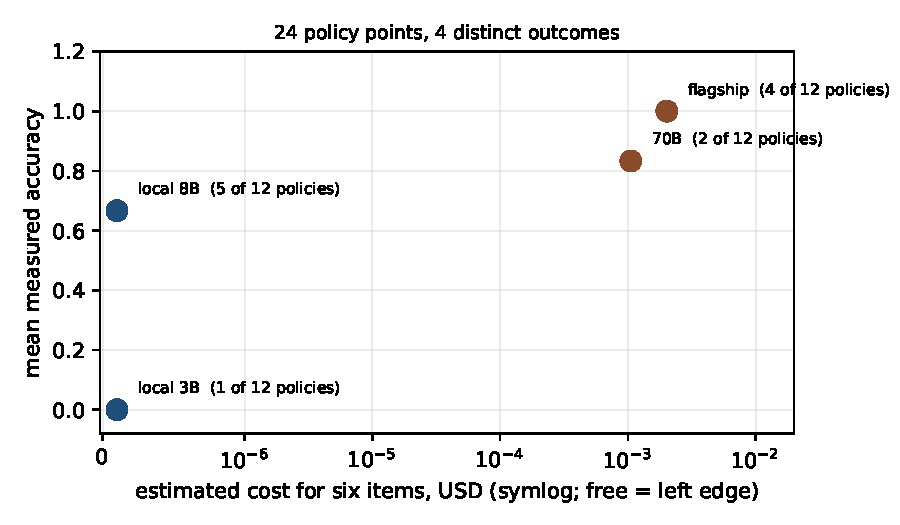
\includegraphics[width=0.92\linewidth]{fig2_sweep.pdf}
\caption{Twelve \code{allow\_flagged} policy points collapse onto four outcomes: schema floor
0.9 forces the flagship at any accuracy floor; with the schema floor released, the accuracy floor
selects 3B, 8B or 70B. All 24 sweep points cost \$0 because nothing is called.}
\end{figure}

Three findings matter. (i) The two thresholds are not interchangeable: the schema floor alone
forces the most expensive arm, and for code items ``schema compliance'' means only that the
program printed a parseable JSON object --- a weaker guarantee than its name suggests, carrying
the larger price. (ii) The cost of a quality floor is uniform and large: exactly 40$\times$ the
cheapest measured cloud arm across all six items, because it is a price ratio, not a token
effect. (iii) Coverage is the health metric: one arm of six still has no measurement, and while
it is never the cheapest and so never wins, the ``refuse versus allow unmeasured'' setting changes
the candidate set at every point without changing a single outcome --- a knob that looks
consequential and is not.

\subsection{Does the policy algebra earn its complexity?}
\label{sec:baselines}

A reviewer should ask what the gates buy. We replay every strategy over the same frozen
per-arm rows --- no new model calls --- on the six computation items where the routed arm
actually ran. Router rows marked \emph{dry-run} are what the current policy would choose,
scored by the measured accuracy of the chosen connection rather than by a new answer.

\begin{table}[h]
\centering
\small
\begin{tabular}{@{}lrrr@{}}
\toprule
\textbf{Strategy} & \textbf{Accuracy} & \textbf{Cost (6 items)} & \textbf{\$ / correct field} \\
\midrule
always local 3B                        & 0.00 & \$0         & -- \\
always local 8B                        & 0.73 & \$0         & \$0 \\
cheapest cloud arm                     & 0.45 & \$0.000489  & \$0.000098 \\
always 70B                             & 0.82 & \$0.002520  & \$0.000280 \\
always flagship                        & 1.00 & \$0.009598  & \$0.000873 \\
capability-only (accuracy, cost ignored) & 1.00 & \$0.009598 & \$0.000873 \\
router, default policy (v9, dry-run)   & 1.00 & \$0.002018  & -- \\
router, same policy before tie-break fix (v8, dry-run) & 0.00 & \$0.002018 & -- \\
router, decisions actually made        & 0.82 & \$0.002542  & \$0.000282 \\
\bottomrule
\end{tabular}
\caption{Baselines on the six computation items. The free 8B is not dominated; the most
expensive arm is; and the v8 row is a defect, not a strategy.}
\end{table}

\begin{figure}[h]
\centering
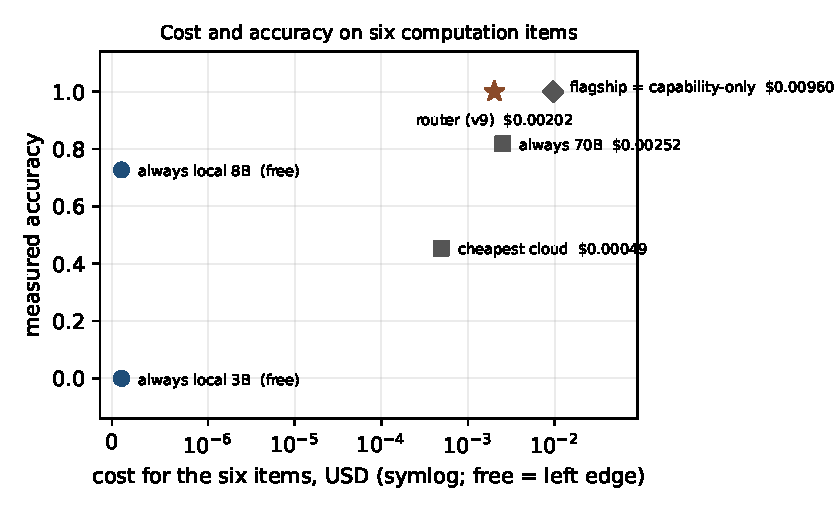
\includegraphics[width=0.92\linewidth]{fig1_cost_accuracy.pdf}
\caption{Cost and measured accuracy for every strategy on the six computation items. Free
models sit on the left edge because \$0 cannot be plotted on a log axis; they are labelled
rather than nudged to a fake price. The router's point is expected accuracy from frozen
measurements, not a new answer.}
\end{figure}

Four readings. (i) \textbf{The free 8B is not dominated}: 0.73 accuracy at \$0 beats the cheap
cloud arm on both axes and loses to the 70B on accuracy alone. (ii) \textbf{Always-big is
dominated}: 1.00 for \$0.0096 is 4.8$\times$ what the default policy pays for the same 1.00, and
capability-only ignores cost and lands there too. (iii) \textbf{Routing was coverage-limited,
not algebra-limited}: the decisions actually made scored 0.82 for \$0.0025 because they were
taken when only three arms had measurements, so the policy fell through to an unmeasured 70B ---
the baseline makes that visible where the sweep alone did not. (iv) \textbf{A defect surfaced
only because the baseline existed}: two arms priced identically (\$2/\$6 chat and reasoning)
tied, the unmeasured one had the lower registration id, and the router chose it. Accuracy 0.00
at \$0.002018. The tie-break now prefers a measured candidate before falling back to id order
(v9); the fix changes accuracy from 0.00 to 1.00 at identical cost, and old policies keep their
original rule so every historical decision still replays.

\subsection{What the log already knew}

Three diagnostics come free from the decision log. \emph{Gate binding}: over 828 decisions the
privacy gate excluded at least one candidate in 26.7\%, verifiability in 62.4\% and emptied the
set 84 times, context fit in 1.6\%, and availability ran in only two decisions and excluded none
--- a gate that never binds
is a gate whose cost is unmeasured, and saying so is more useful than implying all four are
load-bearing. \emph{Latency}: the 70B's median attempt is 2.6\,s, the free local 3B's is 8.3\,s,
and the cheap cloud arm's is 1.5\,s, so ``local is cheaper'' is true and ``local is faster'' is
not --- a trade-off the router makes visible rather than hides. \emph{Determinism}: routing the
same frozen request twice yields records identical in all ten semantic fields, differing only in
id and timestamp.

\subsection{Resilience: ten acceptance checks}

The failure contract is tested against a local HTTP server whose behaviour is switched per model,
so the real transport, retry classification and breaker are exercised rather than mocked.
Table~\ref{tab:accept} gives the results.

\begin{table}[h]
\centering
\small
\begin{tabular}{@{}p{0.06\textwidth}p{0.62\textwidth}p{0.24\textwidth}@{}}
\toprule
\# & Check & Result \\
\midrule
1 & dead endpoint $\rightarrow$ typed refusal naming connection and class & pass \\
2 & 3 failures $\rightarrow$ breaker skips with \code{unhealthy} & pass \\
3 & auth and missing-model not retried; timeout retried twice & pass \\
4 & malformed body escalates, no crash & pass \\
5 & 12 concurrent requests leave a valid chain, 12 unique ids & pass \\
6 & privacy holds over failed attempts (strict profile) & pass \\
7 & one connector class serves a real local and a real cloud endpoint & pass \\
8 & a malformed entry still boots and routes the rest & pass \\
9 & no shadow price; local route costs exactly \$0 & pass \\
10 & audit passes 17/17 on a log produced by the new code & pass \\
\bottomrule
\end{tabular}
\caption{Acceptance checks. Check 7 spent \$0.0002 against a live provider; every other check is
local and free.}
\label{tab:accept}
\end{table}

Check 7 deserves a note. The listing endpoint called the account's 70B model available; a real
call revealed the account could not use it. We therefore changed the health check from a listing
to a one-token completion, because ``listed'' is not ``callable'' --- and that is the same lesson
as the paper's thesis, one layer down.

\section{Limits}
\label{sec:limits}

\paragraph{Statistical power.} Capability cells have six items; one correct answer moves accuracy
by 0.17 and can flip an eligibility verdict. Repeating the battery three times takes the cells to
n = 18 and leaves every mean unchanged for the deterministic arms --- useful as a noise bound,
useless as a substitute for more items. The classifier battery has 44 prompts; the measured
improvement is $p=0.0625$ under an exact paired test. We report the direction, not a population
claim, and the fix is more items from independently labelled corpora, not more analysis of these.

\paragraph{One human annotator, two model annotators, and a classifier that does not generalise
(under the optional rules profile).}
The privacy labels are the author's judgement, frozen before the run; the two further raters of
Section~\ref{sec:annotator} are models, not people, and both reproduce the labels ($\kappa$ 0.97).
``Private'' is a policy choice, not a fact about the world. The ruleset was revised against the
tuning battery, so its 0.98 there is a regression test; on a 64-item held-out battery written after
the freeze it scores \textbf{0.672} with no under-classifications but 58\% of prompts matching no
rule, and on a 72-item second held-out battery from unseen domains it scores \textbf{0.542} with
seven under-classifications. That is the layer's largest weakness, it is measured rather than
suspected, and it is
scoped to the classifier --- the gate itself is exact given a class.

\paragraph{Privacy is a policy, not a guarantee.} Under the shipped default a private request may
reach a cloud endpoint, with a warning on the record. The architecture guarantees that the router
follows the declared policy and that any sensitive cloud route is recorded; it does not guarantee
that the policy is wise, and it cannot protect a user from their own declaration. The strict
profile remains available and is what the mechanism experiment uses.

\paragraph{Prices and availability are the user's declarations.} Migrated prices come from a
pre-RC provider snapshot taken on 2026-10-22 and are marked as declarations rather than
measurements. Providers and keys change under the system: during this work a model was retired,
a key was invalidated twice, and a provider blocked third-party-hosted models for the account
--- each surfaced as a typed error, none anticipated by the design.

\paragraph{Capability is budget-scoped.} Every capability row fixes an output-token budget, and
the same cheap reasoning arm scores 0.22 at 2{,}048 and 1.00 at 8{,}192 on identical items. Our
matrix uses one budget throughout, so no result here says which model is better in general --- only
which is better \emph{at this budget}. Re-measuring at a second budget would double the matrix and
is the obvious next experiment, not a detail to wave away.

\paragraph{Scope of the harness.} Code execution is a guardrail (throwaway directory, scrubbed
environment, import allowlist, timeout), not a sandbox. It exists so the experiment can measure
whether a generated program runs and prints the right value; executing model-written code in a
product is a permissions problem this layer does not solve.

\paragraph{Two local windows.} The local arms cannot hold the large files in context at all, so
the in-context arm of Table~3 has three rows, not five. That is a property of the deployment, not
of the models.

\section{Threats to validity}

\emph{Internal.} The same author wrote the battery, the grader and the analysis. The grader defect
reported above is the concrete instance; the mitigations are that labels were frozen before runs,
that the audit recomputes from raw artifacts with a separately written path, and that the
regrade was mechanical and bounded (it changed exactly the eight rows its rule predicts).

\emph{External.} The models, prices and providers are a 2026 snapshot; two of the five cloud arms
have already changed availability. The routing questions are representative of an assistant that
reads spreadsheets, but not of long-horizon agents.

\emph{Construct.} Accuracy on a small frozen battery is a proxy for usefulness. We deliberately
pair every arithmetic item with a code variant, and we report cost per correct field rather than
cost per token, but neither removes the proxy problem.

\section{Conclusion}

Routing is where an assistant's cost, quality and privacy are actually decided, and it is
usually the least auditable part of the stack. We built a router whose policy is data and whose
decisions are evidence, and we held it to the standard that implies: every number recomputed from
frozen artifacts by a separate script, every failure typed, every claim --- including the ones
that weaken the story --- in the record. The layer routes to a model that scores 1.00 on a task
for about \$0.0003, or to a free model that scores 0.00, depending on a policy file; it computes an
800-row total correctly four times out of five when it writes code and never when it does not;
and it will refuse to answer when the only permitted endpoint is dead, while proving that the
user's content never reached the endpoint it was not allowed to reach. None of that is a claim
about intelligence. All of it is a claim about accountability, and every one of them can be
checked by someone who does not trust us.

\paragraph{Artifacts.} Frozen batteries, raw runs, derived numbers, the audit and the spine are in
\code{05-model-router/} of the DeeWaanAI repository. The spine is the entry point: if it exits
non-zero, no number in this paper should be believed.

\section*{AI-usage disclosure}

This layer was built in human-directed sessions with AI coding assistants (Kimi, Moonshot AI;
with earlier sessions using other assistants), and this paper's method makes that involvement
part of the record rather than a footnote.

\paragraph{What the AI did.} Literature search and citation verification (all 45 review
citations resolved programmatically against OpenAlex/arXiv); code generation for the router, the
store, the audit and the experiment harnesses; battery drafting under instruction; and the
analysis scripts including the spine. Two model annotators (Qwen3.8, DeepSeek-V4.1) served as
the second and third raters of Section~\ref{sec:annotator} --- that role is measured in the
paper, not only disclosed here.

\paragraph{What the AI did not do.} No AI system made an unsupervised design, policy or
publication decision. The gate order, the policy-as-data design, the simplification to a
user-owned connect list, the shipped classifier default, and every spend decision were the
author's, taken in writing (the numbered deltas and owner decisions are in the spec's decision
log). Batteries and labels were frozen before runs; the author approved every cloud call under a
\$10 cap.

\paragraph{Oversight episodes.} Four are on the record, each caught by the verification layer
rather than by inspection: (i) the grader matched answer keys by name and scored correct
programs half-wrong --- found by the spine, fixed by a bounded regrade (Section~\ref{sec:code});
(ii) the audit verified the hash chain but not that the data file matched it --- found by fault
injection, fixed by replaying history against disk (Section~\ref{sec:faultinj});
(iii) a tie-break silently
preferred an unmeasured model --- found by the baseline table, fixed in policy v9
(Section~\ref{sec:baselines}); (iv) an earlier draft of this paper stated ``226 checks'' where the frozen
verification summary now records 263 --- found while building this paper's claim map, corrected
here; and (v) the same draft's classifier-options table carried three rows (0.500, 0.931, and the
``residual cases'' reading) that traced to no frozen artifact; re-measurement under the shipped
contract changed every one of them (Table~\ref{tab:classifier}). Each episode is the same lesson: the artifact, not the assistant, is the source of truth.

\paragraph{Enforcement artifact.} Every number in this paper is registered in
\code{paper/claim\_map/datapoints.json} with a pointer to the frozen raw artifact that carries
it, and \code{verify\_two\_way.py} exits non-zero if any value or any quoted sentence drifts.
The semantic map \code{semantic-claims.json} records what each risky claim means and the
evidence behind it. Both are part of the submission.

% ---------------------------------------------------------------------------
% References verified by paper/verify_citations.py on 2026-10-25: all 15 DOIs resolve.
% For arXiv DOIs the resolved title and first author were compared against the review's
% metadata and match. Non-arXiv DOIs (ACM, NeurIPS, ACL, Zenodo) are verified by resolution;
% their landing pages block automated clients, so titles were not re-derived.
% ---------------------------------------------------------------------------
\begin{thebibliography}{99}
\bibitem{frugal} L.~Chen, M.~Zaharia, J.~Zou. FrugalGPT: How to Use Large Language Models While Reducing Cost and Improving Performance. arXiv, 2023. \texttt{doi:10.48550/arXiv.2305.05176}
\bibitem{mot} M.~Yue, J.~Zhao, M.~Zhang, et al. Large Language Model Cascades with Mixture of Thoughts Representations for Cost-efficient Reasoning. arXiv, 2023. \texttt{doi:10.48550/arXiv.2310.03094}
\bibitem{routellm} I.~Ong, A.~Almahairi, V.~Wu, et al. RouteLLM: Learning to Route LLMs with Preference Data. arXiv, 2024. \texttt{doi:10.48550/arXiv.2406.18665}
\bibitem{hybrid} D.~Ding, A.~Mallick, C.~Wang, et al. Hybrid LLM: Cost-Efficient and Quality-Aware Query Routing. arXiv, 2024. \texttt{doi:10.48550/arXiv.2404.14618}
\bibitem{routerbench} Q.~J.~Hu, J.~Bieker, X.~Li, et al. RouterBench: A Benchmark for Multi-LLM Routing System. arXiv, 2024. \texttt{doi:10.48550/arXiv.2403.12031}
\bibitem{automix} P.~Aggarwal, A.~Madaan, A.~Anand, et al. AutoMix: Automatically Mixing Language Models. NeurIPS, 2024. \texttt{doi:10.52202/079017-4164}
\bibitem{unified} J.~Dekoninck, M.~Baader, M.~Vechev. A Unified Approach to Routing and Cascading for LLMs. arXiv, 2024. \texttt{doi:10.48550/arXiv.2410.10347}
\bibitem{agreement} S.~Kolawole, D.~Dennis, A.~Talwalkar. Agreement-Based Cascading for Efficient Inference. arXiv, 2024. \texttt{doi:10.48550/arXiv.2407.02348}
\bibitem{tasktype} J.~Lee. Most of the LLM Routing Gap Is Task Type. arXiv, 2026. \texttt{doi:10.48550/arXiv.2608.23023}
\bibitem{privcascade} K.~Zhang, C.~Wang, L.~Peng. Privacy-preserved LLM Cascade via CoT-enhanced Policy Learning. arXiv, 2024. \texttt{doi:10.48550/arXiv.2410.08014}
\bibitem{edgesurvey} S.~Li, H.~Wang, W.~Xu, et al. Collaborative Inference and Learning between Edge SLMs and Cloud LLMs: A Survey of Algorithms, Execution, and Open Challenges. ACM Computing Surveys, 2026. \texttt{doi:10.1145/3838593}
\bibitem{verifier} M.~Yao, Z.~Zhang, S.~Li, et al. VeriRouter: Towards Verifiable LLM Routing. arXiv, 2026. \texttt{doi:10.48550/arXiv.2610.17431}
\bibitem{structout} C.~Galeone, M.~Park, G.~Ettorre. When Correct Isn't Usable: Improving Structured Output Reliability in Small Language Models. arXiv, 2026. \texttt{doi:10.48550/arXiv.2605.02363}
\bibitem{auditroute} F.~Barcelos. Deterministic and Auditable Routing for Artificial Intelligence in Regulated Environments. Zenodo, 2026. \texttt{doi:10.5281/zenodo.20531686}
\bibitem{rome} H.~Tang, Y.~Yan, J.~Lu, et al. Route to Rome Attack: Directing LLM Routers to Expensive Models via Adversarial Suffix Optimization. ACL, 2026. \texttt{doi:10.18653/v1/2026.acl-long.2051}
\bibitem{qafiya} Y.~Hariri. Qafiya: a provenance-first data substrate (Layer 1 specification and implementation). DeeWaanAI, 2026.
\end{thebibliography}

\end{document}
